\documentclass{sbrt2013port}
%\usepackage[brazil]{babel}
\usepackage{amsmath}
\usepackage{amssymb}
\usepackage{graphicx}
\usepackage{color}
%\usepackage{placeins}
\usepackage{bm}
%\usepackage{cite}
%\usepackage{stfloats}
%\usepackage{float}
\usepackage{hyperref}
%\usepackage{cite}
\usepackage{tabularx,colortbl}


\begin{document}

\title{Simulating Generalized Fading Channels in Python}

\author{Jos� Vin�cius de M. Cardoso$^1$,   Paulo Ribeiro Lins J�nior$^2$, Wamberto Queiroz$^1$ e Marcelo Sampaio de Alencar$^3$
\thanks{\noindent Instituto de Estudos Avan�ados em Comunica��es -- Iecom; $^1$Universidade Federal de Campina Grande -- UFCG; $^2$Grupo de Pesquisa em Comunica��es e Processamento de Informa��o -- GComPI/Instituto Federal de Educa��o, Ci�ncia e Tecnologia da Para�ba -- IFPB, Campus Campina Grande -- PB, $^3$Universidade Federal da Bahia -- UFBA, emails: $^1$\{josevinicius, wamberto\}@iecom.org.br, $^2$paulo.lins@ifpb.edu.br e $^3$malencar@iecom.org.br.}}

\maketitle

\markboth{XXXVI SIMP�SIO BRASILEIRO DE TELECOMUNICA��ES E PROCESSAMENTO DE SINAIS - SBrT'2018, 16-19 DE SETEMBRO DE 2018, CAMPINA GRANDE, PB} {XXXVI SIMP�SIO BRASILEIRO DE TELECOMUNICA��ES E PROCESSAMENTO DE SINAIS - SBrT'2018, 16-19 DE SETEMBRO DE 2018, CAMPINA GRANDE, PB}

\begin{abstract}
    We present a novel and well tested Python-based library for simulating and computing
    generalized fading channels, considering $\alpha\text{-}\mu$, $\kappa\text{-}\mu$, and
$\eta\text{-}\mu$ distributions. We describe the
    applicability of this library using a few communications channels scenarios
    impaired by generalized fading, namely, spectrum sensing and bit error
    rate computation. The development of the library is open source and its code, along
    with examples, are available at
    \texttt{http://github.com/mirca/maoud}.
\end{abstract}

\begin{keywords}
Generalized Fading, Simulation, Python
\end{keywords}

\section{Introduction}

The study of modern wireless communications systems heavily relies on fading channel simulation.
By fading channel simulation, we refer to the generation of samples from a probability distribution
that resembles the effects and impairments caused by real communications fading channels on the
transmitted signal.

Although accurate and precise distributions for generalized fading have been
estabilished in the literature, such as $\alpha\text{-}\mu$~\cite{yacoub.2007.1},
$\kappa\text{-}\mu$~\cite{yacoub.2007.2} and $\eta\text{-}\mu$~\cite{yacoub.2007.2},
the generation of samples following these distributions is usually
a time-consuming task.

In~\cite{cogliatti2012}, the authors built an efficient
algorithm, based on the rejection method, for generation of samples from those
distributions. However, there are neither open nor
closed source implementations available to the scientific community.

In this paper, we present an open source Python package
for generation of samples following the $\alpha\text{-}\mu$, $\kappa\text{-}\mu$, and
$\eta\text{-}\mu$ distributions. The usefullness of ths package is illustrated
through well known examples involving spectrum sensing and bit error rate (BER) computation.

\section{Rejection Sampling}\label{rejec}

The algorithm implemented in this work, originally proposed in~\cite{cogliatti2012},
is based on the rejection method, which is one of the most used for the generation
of samples of a probability distribution.

We briefly describe the algorithm as follows. Consider that we would like to simulate a
random variable $x$ with a probability density $f$. The basic idea is to find
an alternative probability density $g$, from which there exists an efficient procedure
to generate samples, e.g., inverse methods. Additionally, it is required that $g$
majorizes $f$, i.e., we assume that there exists a real number $c$ such that $f(x)/g(x) < c$.

Basically, the steps of the rejection algorithm are~\cite{ross}:
\begin{enumerate}
	\item generate a sample $y$ from the probability density $g$;
    \item generate a sample $u$ from a uniform density with support $(0, 1)$;
	\item check $u \leq \frac{f(y)}{cg(y)}$; if true then accept $y$; otherwise, return to step 1.
\end{enumerate}

The implementation of this algorithm along with the code to efficiently generate
samples from the $\alpha$-$\mu$, $\eta$-$\mu$, and $\kappa$-$\mu$ distributions
is available at \url{http://github.com/mirca/maoud}.

In order to validate the implementation, we apply the routines to
two use cases in wireless communications: spectrum sensing and bit error rate computation.

\section{Spectrum Sensing in Complex Generalized Fading Channels}~\label{sensing}

The spectrum sensing problem consists in deciding whether or not a given channel
frequency band is being occupied by a licensed (primary) user and, in case that such
frequency band is available, how to opportuniscally allocate secondary users
such that the interference on the primary user is negligible.

From a probabilistic point of view, the spectrum sensing problem may be framed as
a decision theory problem, as follows
\begin{align}
    H_0:  \bm{y} &= \bm{w},\\
    H_1:  \bm{y} &= h\bm{s} + \bm{w},
\end{align}
\noindent in which $\bm{y} \in \mathbb{C}^{n\times 1}$ is the received vector signal,
$\bm{w} \in \mathbb{C}^{n\times 1}$ is complex Gaussian noise process with zero mean
vector and covariance matrix given as $\sigma^2\bm{I}_n$, and $h$ is the channel gain.

In~\cite{cardoso2017}, the authors have shown that the cumulative distribution function (cdf) of the
energy statistic $\tilde{y} \triangleq \bm{y}^{\dagger}\bm{y}$ conditioned on the knowledge of $h$,
in case that $\bm{s}$ is an $M$-PSK signal such that every symbol has the same probability of occurrence,
$\mathbb{P}(s_n = s) = \frac{1}{M}$, is given as
\begin{align}
    P(\tilde{y} | h, H_1) = 1 - \mathrm{Q}_{n}\left(\sqrt{\dfrac{2n|h|^2E_s}{\sigma^2}}, \sqrt{\dfrac{2\tilde{y}}{\sigma^2}}\right),
\end{align}
in which $\mathrm{Q}_{n}$ is the Marcum-$\mathrm{Q}$ function and $E_s$ is the energy per symbol.

Recall that the energy detection rule can be expressed as
\begin{equation}
    d_\delta (\tilde{y}) = \mathbb{I}(\tilde{y} > \delta)
\end{equation}
in which $\mathbb{I}$ is the indicator function, $\delta$ is a strictly positive real
number known as energy threshold, and $d_\delta (\tilde{y}) = j,~j \in \{0,1\}$,
means that the detector has decided in favor of the hypothesis $H_j$.

As a result, the probabilities of false alarm and miss detection can
be written as
\begin{align}
    \mathbb{P}\left(d_\delta(\tilde{y}) = 1 | H_0\right) &=
        1 -  P(\delta | H_0) = 1 - \gamma\left(n, \frac{\delta}{\sigma^2}\right),\label{eq:pf} \\
    \mathbb{P}\left(d_\delta(\tilde{y}) = 0 | H_1\right) & = \int_{-\infty}^{+\infty} P(\delta | h, H_1)p(h)\;\mathrm{d}h,\label{eq:pd}
\end{align}
in which $\gamma$ is the regularized lower incomplete Gamma function, $p(h)$ is the pdf of the fading,
and $\delta$ is the energy detection threshold.

The performance of detection schemes can be measured by computing the Receiver Operating
Characteristic (ROC), which consists in varying $\delta$ and computing the pairs of
probability of false alarm and miss detection, as illustrated in Fig.~\ref{fig:spectrum-sensing}, in which the solid curve represents the theorectical probabilities as stated on
(\ref{eq:pf}) and (\ref{eq:pd}) for different values of
$\delta$, whereas bullets represent Monte Carlo simulations acquired with $10^6$ realizations.
The input signal $\bm{s}$ consists in a vector of length $n=25$ in which each entry represents
a symbol of a 64-PSK constellation. Symbols are assumed to be equiprobable and
the signal-to-noise ratio is set to $5$ dB.

\begin{figure}[!htb]
    \centering
    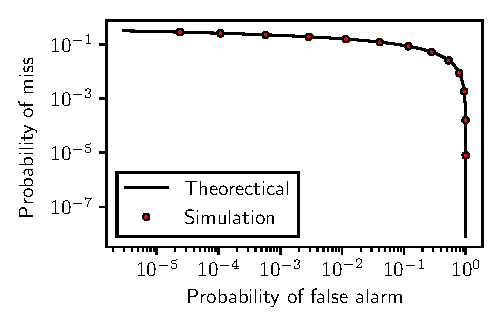
\includegraphics{figures/spectrum_sensing}
    \caption{Receiver Operating Characteristic for the energy detector in $\alpha$-$\mu$
             channel with $\alpha=2$ and $\mu=1$.
             }
    \label{fig:spectrum-sensing}
\end{figure}

\section{Bit Error Rate in $\alpha$-$\mu$ Fading}~\label{ber}

Consider the system
\begin{align}
    y = hs + w
\end{align}
in which $s \in \{0, a\}$, $a \in \mathbb{R}_{+}$, is a transmitted signal,
$h$ is an $\alpha$-$\mu$ random variable and $\bm{w}$ is a Gaussian random variable
with zero mean vector and variance $\sigma^2$, and $y$ is the received signal.

Assume that the binary symbols are equiprobable, then the probability of one bit error
is given as
\begin{align}
    p_{e} = \dfrac{1}{2}\left(\mathbb{P}\left(\hat{y} = 0 | s = a\right)
                            + \mathbb{P}\left(\hat{y} = 1 | s = 0\right)\right).
\end{align}

Further, assume that the decoded bit $\hat{y}$ is estimated using the minimum distance decoding
rule, i.e.,
\begin{align}
    \hat{y} = \mathbb{I}(|y - a|^2 < |y|^2)
\end{align}
therefore
\begin{align}
    \mathbb{P}\left(\hat{y} = 1 | s = 0\right) & = \mathbb{P}\left(|w - a|^2 - |w|^2 < 0\right) = 1 - \Phi\left(\frac{a}{2\sigma}\right)
\end{align}
and likewise
\begin{align}
    \mathbb{P}\left(\hat{y} = 0 | s = a\right) & = \mathbb{P}\left(ha + w < \frac{a}{2}\right) = \mathbb{E}_h\left(\Phi\left(\frac{a(1 - 2h)}{2\sigma}\right)\right).
\end{align}

In Fig.~\ref{fig:ber}, we show the expression of the BER as a function of the signal-to-noise ratio,
for the system under consideration with $\alpha=2$ and $\mu = 5$.
As we can see, the simulation presents an excellent agreement against theorectical results.
\begin{figure}[!htb]
    \centering
    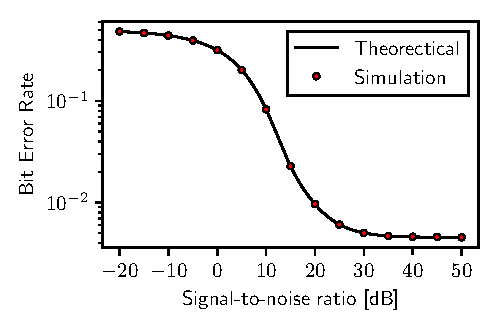
\includegraphics{figures/ber}
    \caption{BER as a function of the SNR for $\alpha=2$ and $\mu = 5$}
    \label{fig:ber}
\end{figure}

\section{Conclusions}\label{conclusions}

This paper presents a novel Python-based library for generalized fading simulation.
The implementation is tested and validated in two use cases, namely,
spectrum sensing and BER computation.

The computational results show that the implementation presents a
satisfactory agreement when compared with the theorectical formulation.

We expect that the proposed library, which is open source,
will be usefull to researchers, professors, and students of
the field of wireless communications.

Finally, all the simulations were done in a personal laptop,
and the generation of $10^6$ samples from any of the generalized fading
distributions took on average 10 seconds.

\bibliographystyle{IEEEtran}
\bibliography{manuscript}

\end{document}
